\documentclass[12pt, a4paper]{article}
\usepackage[swedish]{babel}
\usepackage[version=4]{mhchem}
\usepackage{amsmath}
\usepackage[swedish]{varioref}
\usepackage{hyperref}
\hypersetup{
    colorlinks=true,
    linkcolor=black,
    pdftitle={Fysik 1 Uppslagverk},
    pdfpagemode=FullScreen
}
\usepackage[swedish]{cleveref}
\usepackage{amsthm}
\renewcommand\qedsymbol{V.S.V.}
\theoremstyle{definition}
\newtheorem{exm}{Exempel}
\usepackage{cancel}
\usepackage{float}
\usepackage{array}
\usepackage{enumitem}
\renewcommand{\labelitemii}{$\circ$}
\usepackage[margin=2.5cm]{geometry}
\usepackage{pgf}
\usepackage{tikz}
\usepackage{graphicx}
\usetikzlibrary{bending}
\usepackage{tcolorbox}
\tcbuselibrary{theorems}
\usepackage{array}

% Make the heart character work
\DeclareSymbolFont{extraup}{U}{zavm}{m}{n}
\DeclareMathSymbol{\varheartsuit}{\mathalpha}{extraup}{86}


\title{Sammanfattning - Fysik 1 \\ Blackebergs Gymnasium}
\author{Marcell Ziegler - NA21D}

\newcommand{\noref}{\textcolor{red}{\textbf{\textit{\underline{missing reference}}}}}

\begin{document}
    \begin{titlepage}
        \maketitle
        \centering
        \vfill
        
\includegraphics[width=0.6\textwidth]{title.jpg}
        \vfill
        \textbf{OBS!} Alla siffror/referenser som verkar vara länkar är antagligen länkar. Svåra/ogenomgångna matte-symboler borde också vara länkar som leder till förklaring, dock endast for första uppkomsten per ekvation. Tryck gärna om du undrar nåt!
    \end{titlepage}

    \tableofcontents

    \newpage

    \section*{Förord}
    Innan början finns det några viktiga saker att utreda för denna sammanfattning. Först av allt är detta ett fritidsprojekt och inte skolmaterial, därför finns det ingen garanti på att allt är 100\% rätt dock borde dokumentet överlag inte innehålla några större faktafel. Nästa punkt är att denna sammanfattning är gjord för effektivitet så alla förklaringar är inte fullständiga och huvuddelen innehåller inte fullständiga härledning och heller inte många räkneexempel. Om du söker fullständiga förklaring på vissa saker får du gärna titta i bilagorna mot slutet av dokumentet. Där hittar du även förklaringar till matematiska täcken som jag använder men som vi inte har gått igenom. Jag kommer heller inte förklara vanliga symboler för storheter som ex. massma ($m$) och hastighet ($v$).
    \begin{center}
        \large{Ha kul främst av allt, men kom ihåg likt vad Tor brukar säga:}\\
        \Large{Jag \textcolor{red}{$\varheartsuit$} Fysik!}
    \end{center}

    \part{Rörelse}
    \input{chapters/rörelse.tex}

    \part{Termodynamik}
    Termodynamik är läran om värme och inre energi.
    \section{Inre energi (Värmeenergi)}
Detta är den energin som finns hos oordnad rörelse i materia. Den består av ett två delar:
\begin{itemize}
    \item Rörelseenergi - kommer från aggregationstillstånd och brownisk rörelse
    \item Potentiell energi - kommer från bindningar mellan partiklar som liknar fjädrar
\end{itemize}
Inre energi kan bestå av en eller båda av dessa delar dock består den av båda i de allra flesta fall. Inre energi har enheten Joule (J).
\subsection{Värme}
Värme är inre energi som övergår från varmt till kallt av sig själv. Det är alltså inte energi i sig utan dessa övergång från en temperatur till en anna som vi känner av när vi nuddar någonting kallt eller varmt. Föreställ dig att du är i ett vakum där allt är lika kallt och du inte har någon kroppsvärme. Då skulle du inte kunna känna av kylan då det inte finns en referenspunkt. Om du hade kroppsvärme hade frusit väldigt mycket då mycket av din energi övergår till den kalla omgivningen vilket upplevs som kallt.
\subsubsection{Värmeöverföring}
Här har vi kärnan av dett ämne inom fysiken och dess namne. Här följer de 3 främsta sättet som värme överförs.
\begin{enumerate}
    \item Ledning
    \item Strålning
    \item[(3.] Konvektion)
\end{enumerate}
Den sista står inom parantes då den egentligen är ledning under spefika omständigheter men den brukar räknas som ett självständigt sätt ändå. Här är förklaringarna:
\subsubsection*{Ledning}
Detta är när värme överförs mellan två föremål som befinner sig i kontakt med varandra. Detta sker eftersom partiklarna i rörelse kolliderar med varandra och sprider deras rörelseenergi och därmed sin värme. I slutändan kommer två föremål i kontakt alltid att anta en jämn fördelning av värmeenergi genom hela föremålet givet nog med tid. Detta går mycket långsamt för föremål som är goda isolatorer och mycket snabbt för bra ledare.
\subsubsection*{Strålning}
Detta är överföring av värme genom Infraröd (IR) elektromagnetisk (EM) strålning. Detta är ljus, dvs. fotoner, som befinner sig i IR-spektrat. Det må vara ljus, men det är osynligt ljus. Denna metod kräver ingen fysisk kontakt mellan två föremål. Alla föremål avger någon typ av IR-strålning som en konsekvens av deras inre energi dock är denna mängd ofta mycket liten i relation till andra källor i omgivning och märks därför oftast enbart från föremål dedikerade till värmeproduktion som en spis, solen och en värmelampa.
\subsubsection*{Konvektion}
Denna process är när luft eller annan gas värms vid en punkt och sedan sprider sig i dess omgivning på grund av att varm luft är lättare än kall luft. När den har tappat sin värme genom strålning och ledning kommer den att falla ner och bli kall. Denna cykliska egenskap hos gas som värms vid en punkt och sedan låts cirkulera kallas \emph{konvektion}. Som sagt är detta inte ett självständigt sätt att överföra värme men ses som unikt nog att få sitt egna namn. Många element i hus baseras på konvektion. Det är mycket mer effektivt att låta luften transportera värmen till dess destination än att försöka värma varje punkt i ett utrymma då räckvidden av ledning är låg och strålning är mycket ineffektivt.

\subsection{Temperatur}
Detta är ett mått på den genomsnittliga rörelseenergi hos partiklarna i föremålet. Det finns flera mått på temperatur men SI-enheten är Kelvin (K). 0 K är den så kallade \emph{absoluta nollpunkten} alltså den temperatur där rörelseenergi i ett föremål är 0. Andra enheter är grader Celcius (\degC) och grader Fahrenheit ($\mathrm{^\circ F}$). Fahrenheit är hemskt och behandlas varken i denna kurs eller någon anna du kommer hitta inom Europa. Celcius å andra sidan har många likheter med Kelvin. En skillnad på 1 K motsvarar en skillnad på 1\degC. 0\degC\ är dock inte samma som 0 K så de kan tyvärr inte ersätta varandra. 0\degC\ motsvarar fryspunkten för vatten vilket ger att$0^\circ \mathrm{C} = 273.15\,\mathrm{K}$ och $T_{\mathrm{K}} = T_{^\circ \mathrm{C}} - 273.15$.

Det är mycket viktigt att notera att temperatur enbart är en av de två typerna av inre energi. Detta innebär att den inre energi kan förändras utan att temperaturen gör det. Utöver detta kan vi se att rörelseenergi är den enda typen av inre energi som kan ''smitta av sig'' dvs. överföras. Andra typer av inre energi kan inte överföras utan förblir bundna i ämnet. En annan viktig egenskap av temperatur är att det bestämmer vilket håll värmet flödar. Saker med låg temperatur ''suger åt sig'' värme medan varma föremål avger värme. Detta bevisar återigen att enbart rörelseenergi påverkar temperaturen då bara rörelseenergi kan ''smitta av sig'' till andra föremål.

\section{Aggregationstillstånd}
Ett ämnes faser eller \emph{aggregationstillstånd} är det olika konfigurationer som dess materia kan anta. I de allra flesta fall finns det tre faser av materia men i vissa omständigheter finns det fyra. De främsta tre kommer täckas av denna kurs men det är bra att veta om den fjärde också. Fasernas namn och namn på övergångarna mellan de är som följande:
\begin{center}
    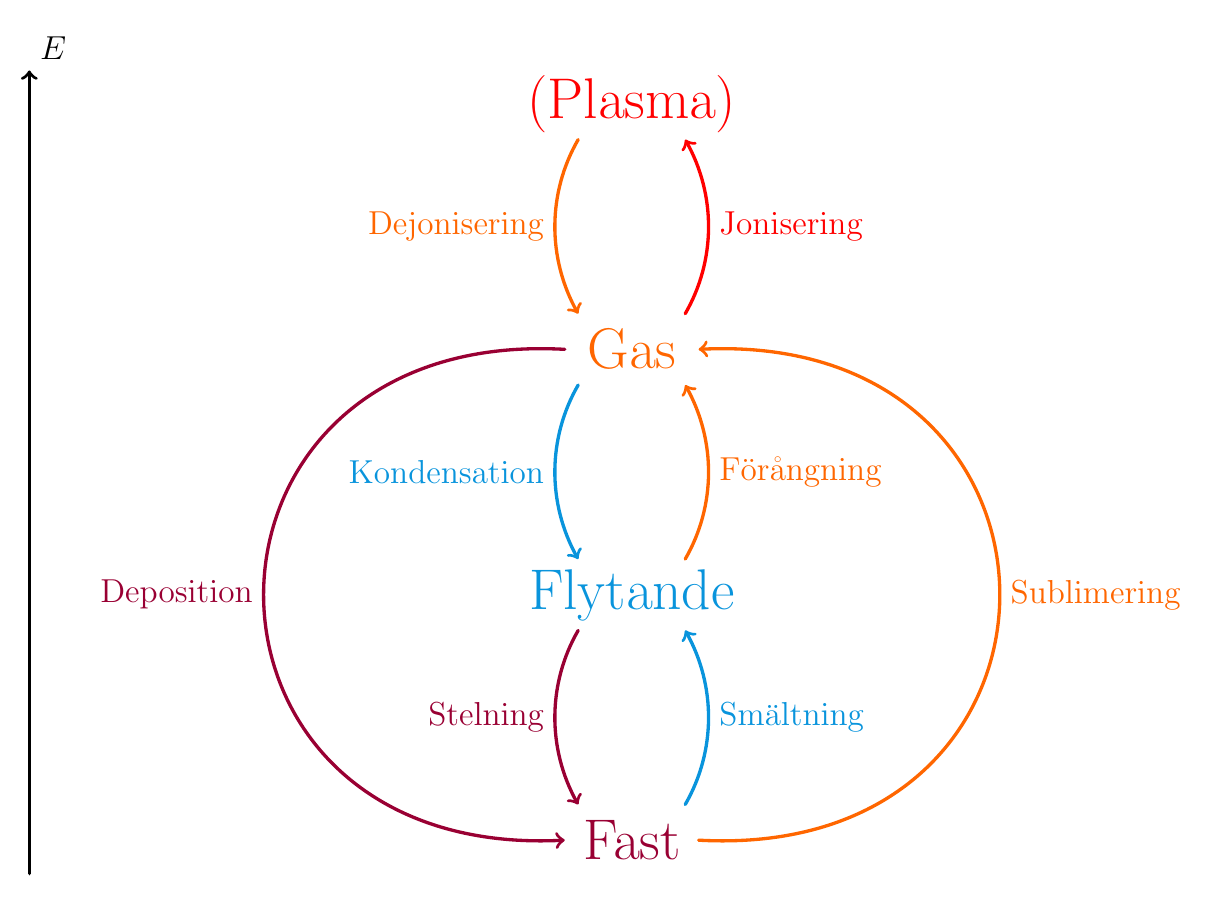
\begin{tikzpicture}[every path/.style={line cap=round, very thick}, scale=0.85]
        \draw[->] (-9,-6) -- ++(0,12) node [anchor=south west] {\large{$E$}};
        %Phases
        \node[color=purple!80!black] at (0,-5.5) {\huge{Fast}};
        \node[color=cyan!80!blue] at (0, -11/6) {\huge{Flytande}};
        \node[color=orange!80!red] at (0, 11/6) {\huge{Gas}};
        \node[color=red] at (0, 5.5) {\huge{(Plasma)}};
        %transitions up
        \draw[->, yshift=-1.3cm, xshift=0.8cm, color=cyan!80!blue] (0,-11/3) arc [radius=2.6cm,start angle=330, delta angle=60] node [pos=0.5, anchor=west, align=left] {\large{Smältning}};
        \draw[->, yshift=-1.3cm, xshift=0.8cm, color=orange!80!red] (0,0) arc [radius=2.6cm,start angle=330, delta angle=60] node [pos=0.5, anchor=west, align=left] {\large{Förångning}};
        \draw[->, yshift=-1.3cm, xshift=0.8cm, color=red] (0,11/3) arc [radius=2.6cm,start angle=330, delta angle=60] node [pos=0.5,anchor=west,align=left] {\large{Jonisering}};
        %Transitions down
        \draw[<-, yshift=-1.3cm, xshift=-0.8cm, color=purple!80!black] (0,-11/3) arc [radius=2.6cm,start angle=210, delta angle=-60] node [pos=0.5, anchor=east, align=right] {\large{Stelning}};
        \draw[<-, yshift=-1.3cm, xshift=-0.8cm, color=cyan!80!blue] (0,0) arc [radius=2.6cm,start angle=210, delta angle=-60] node [pos=0.5, anchor=east, align=right] {\large{Kondensation}};
        \draw[<-, yshift=-1.3cm, xshift=-0.8cm, color=orange!80!red] (0,11/3) arc [radius=2.6cm,start angle=210, delta angle=-60] node [pos=0.5,anchor=east,align=right] {\large{Dejonisering}};
        %full range transitions
        \draw[->, color=orange!80!red] (1,-5.5) .. controls (7,-11/6-4) and (7,-11/6+4) .. (1,11/6) node [pos=0.5,align=left,anchor=west] {\large{Sublimering}};
        \draw[<-, color=purple!80!black] (-1,-5.5) .. controls (-7,-11/6-4) and (-7,-11/6+4) .. (-1,11/6) node [pos=0.5,align=right,anchor=east] {\large{Deposition}};
    \end{tikzpicture}
\end{center}

\subsection*{Plasma}
En mycket varm joniserad gas. Hittas exempelvis i stjärnor. Täcks inte av krusen.

\subsection*{Gas}
När de olika formelenheterna av ämnet är i princip obundna till varandra och kan flyta fritt i omgivningen. Detta aggregationstillstånd har högst inre rörelseenergi.

\subsection*{Flytande}
Detta tillstånd, bättre känt som vätska, är det som händer när formelenhetern är löst bundna till varandra. Detta gör att de kan röra på sig occh anpassa sin form för att passa behållaren men är inte lika fria som en gas. Den viktigaste skillnaden är dock att vätskor är okomprimerbara till skillnad från gaser.

\subsection*{Fast}
Detta är när formelenheterna är hårt bundna till varandra är helt orörliga. Det finns många olika sätt att kunna anta fast form. Vissa ämnen bildar kristaller, andra metallbinder bland annat.

\subsection{Energi vid fasövergångar}
De två typerna av fasövergångar som vi kommer att gå igenom i denna kurs är \linebreak $\text{vätska} \longleftrightarrow \text{gas}$ och $\text{fast} \longleftrightarrow \text{vätska}$. De andra som står på diagrammet ovan är enbart där för full korrekthet och kommer inte att behandlas i kursen. För dessa övergångar gäller följande:
\begin{center}
    \begin{tabular}{c l}
        $E = c_s \cdot m$            & Smältvärme vid en specifik smältentalpi $c_s \left[ \frac{\mathrm{kJ}}{\mathrm{kg}} \right]$                           \\
        $E = c_{\textit{å}} \cdot m$ & Ångbildningsvärme vid en specifik ångbildningsentalpi  $c_{\textit{å}} \left[ \frac{\mathrm{kJ}}{\mathrm{kg}} \right]$
    \end{tabular}
\end{center}
Smältvärmen gäller för övergångar fast $\to$ flytande och flytande $\to$ fast. Ångbildningsvärmen kommer gälla för övergångarna flytande $\to$ gas och gas $\to$ flytande. Negativ energi innebär utsläpp energi och uppstår när du rör dig ner på energiskalan (se bild).

Entalpivärdena motsvarar energin att smälta respektiva förånga 1 kg av material och skiljer sig för varje material. Dessa värde hittas i en värdetabell i formelsamlingen. Dessa värden antar naturligtvis konstant tryck. En sista sak att notera är att entalpi känner man igen från kemin där det mäts i $\mathrm{kJ/mol}$ men här har man valt att konvertera detta till ett mått beroende på massa av varje material för att det bättre ska passa in i formler för fysiken. Man kan naturligvis få fram ett värde i $\mathrm{kJ/kg}$ för alla entalpivärden från kemin så länge man vet molmassan av materialet, vilket vi vet.

    \newpage
    \appendix
    \section{Härledningar}
    \label{appendix:härledning}
    \input{chapters/härledningar.tex}
    \section{Exempel}
    \label{appendix:exempel}
\end{document}